\section{Värmeledning}
\label{sec:heatconduction}

Det pågår ständigt värmetransport från varma till kalla objekt. Konduktion, eller värmeledning, innebär att värmeenergi flödar genom ett material, utan att materialet i sig rör sig eller flyttar sig. Värmetransporten är proportionell mot temperaturskillnaden över konstruktionen. Konduktiviteten, eller värmeledningsförmågan, ofta betecknad $k$ inom fysiken eller $\lambda$ inom byggsektorn är en materialegenskap som beskriver hur snabbt en temperaturskillnad utjämnas genom konduktion i enheten $\unit{Wm^{-1}K^{-1}}$. I denna rapport används den förstnämnda symbolen, $k$. För att bestämma $k$ för ett material utsätter man det för en temperaturskillnad och mäter den värmemängd som passerar genom materialet per tidsenhet. Generellt gäller att värmeflödet per ytenhet är $\mathbf{q} = - k \nabla T \unit{Wm^{-2}}$. Detta samband brukar kallas för Fouriers värmelag. För ett homogent material i en dimension förenklas detta till

\begin{equation}\label{eq:conduction:fourier}\boxed{ \; \; \;
q_x = -k \frac{\mathrm{d}T}{\mathrm{d}x} = -\frac{k}{\mathrm{d}}\left( T_2-T_1\right) \unit{Wm^{-2}}
\; \; \; }
\end{equation}

där $d$ betecknar materialets tjocklek och $T_2$ samt $T_1$ är temperaturen i vardera änden av materialet. Begreppet U-värde kan nu införas och definieras som $U = \frac{k}{\mathrm{d}} \unit{Wm^{-2}K^{-1}}$, det vill säga $q_x = U\mathrm{d}T = U\left( T_2-T_1 \right)$. Även R-värdet introduceras och definieras som inversen av U-värdet, alltså $R=1/U \unit{m^2KW^{-1}}$. Dessa två storheter är ofta användbara inom byggfysik och relaterade områden eftersom man med dem exempelvis kan jämföra olika väggars värmeledningsförmåga.

En schematisk bild över en vägg i en dimension som består av $n$ olika material kan ses i figur \ref{fig:staticwallmethod:wall}. Med materialens värmeledningsförmåga, $k_i$, för $i=1,2\,,\,...\,,\,n$ samt längden på elementen, $d_i$, använder vi nu Fouriers värmeledningsekvation för att teckna värmeflödet och temperaturerna $T_i$, i punkterna mellan de olika delarna av väggen med randvillkoren $T_1 = T_H$ samt $T_{n+1} = T_L$.

\begin{figure}[hpbt]
\centering
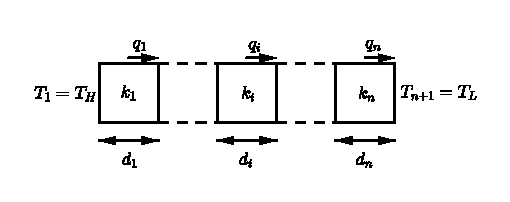
\includegraphics[scale=1.2]{images/wall.eps}
\caption{Schematisk bild över en vägg som består av $n$ olika element med olika
längd och värmeledningsförmåga.}\label{fig:staticwallmethod:wall}
\end{figure}

För varje del av väggen kan vi sätta upp ekvationer från Fouriers ekvation för värmeflöde. Vi får flöde in i en del enligt \eqref{eq:staticwallmethod:rod} och flödet ut genom väggen blir detsamma ty temperaturen är konstant.

\begin{equation}
\label{eq:staticwallmethod:rod}
q_i = -k_i\frac{T_{i+1}-T_{i}}{L_i} \, \Leftrightarrow \, \frac{L_i}{k_i}q_i = T_{i+1}-T_{i}
\end{equation}

Vid statiskt värmeflöde är $q_1 = \, ... \, = q_i = \, ... \, = q_n$, vilket innebär att

\begin{equation}
\sum_{i=1}^n \frac{L_i}{k_i}q_i = q\sum_{i=1}^n \frac{L_i}{k_i} = q\sum_{i=1}^n R_i = \sum_{i=1}^n \left( T_{i}-T_{i+1} \right) = T_H - T_L 
\end{equation}

det vill säga

\begin{equation}
q R_\text{total} = T_H - T_L
\end{equation}

och

\begin{equation}
U_\text{total} = \frac{1}{R_\text{total}} = \frac{1}{\sum_{i=1}^N R_i}.
\end{equation}

Värmeledningsförmågan, och därmed även R- samt U-värden, påverkas av materialets densitet, porositet, temperatur samt fuktighet. Fuktkorrigering görs ibland, enligt vissa framställda värden.

Utifrån Fouriers värmelag kan man härleda ytterligare ett viktigt samband, värmeledningsekvationen. Anta en infinitesimal volym, som varken utsätts för eller utför något arbete relativt omgivningen. Enligt grundläggande termodynamik kan då en godtyckligt liten förändring av värmeenergin (i $\unit{J m^{-3}}$) skrivas som $\mathrm{d}Q = c_p \rho \mathrm{d}T$.  I en dimension, över ett litet tidssteg $t-\mathrm{d}t< \tau < t+\mathrm{d}t$ och en liten sträcka $x-\mathrm{d}x < l < x+\mathrm{d}x$, fås att

\begin{equation}
\mathrm{d}E = c_p \rho \int_{x-\mathrm{d}x}^{x+\mathrm{d}x} \left[ T\left( l, t+\mathrm{d}t\right) - T\left( l, t-\mathrm{d}t\right)\right]dl = c_p \rho \int_{t-\mathrm{d}t}^{t+\mathrm{d}t} \int_{x-\mathrm{d}x}^{x+\mathrm{d}x} \frac{\partial T}{\partial \tau} \mathrm{d}l\mathrm{d}\tau
\end{equation}

Från Fouriers värmelag blir för samma förändring

\begin{equation}
\mathrm{d}E = k\int_{t-\mathrm{d}t}^{t+\mathrm{d}t} \left[ \frac{\partial T}{\partial x}\left( x + \mathrm{d}x, \tau \right) - \frac{\partial T}{\partial x}\left( x-\mathrm{d}x, \tau \right)\right]d\tau =  \int_{x-\mathrm{d}x}^{x+\mathrm{d}x} \frac{\partial}{\partial x} \left( k \int_{t-\mathrm{d}t}^{t+\mathrm{d}t} \frac{\partial T}{\partial x} \mathrm{d}\tau \right)\mathrm{d}l
\end{equation}

Kombinering av dessa och det faktum att det gäller för en godtycklig sträcka $\mathrm{d}l$ samt tid $\mathrm{d}\tau$, vilket innebär att integralen kan tas bort, ger att

\begin{equation}\label{eq:conduction:heateq}\boxed{ \; \; \;
c_p \rho \frac{\partial T}{\partial t} = \frac{\partial}{\partial x} \left( k \frac{\partial T}{\partial x} \right) \Leftrightarrow \frac{\partial T}{\partial t} = \alpha \Delta T
\; \; \; }
\end{equation}

Detta samband brukar kallas för värmeledningsekvationen.

\paragraph{Tröghet}
Det kan förefalla intuitivt att väderförändringar påverkar fastigheter, men hur mycket det spelar roll det egentligen. I det resonemanget spelar termen tröghet en betydande roll. Beroende på hur tjocka väggarna är, samt vilket material de är byggda av spelar de yttre omständigheterna olika stor roll. Trögheten i väggarna är således ett begrepp för hur lång tid det tar innan en väderförändring märks inomhus då yttre parametrarna ändrar sig. En stor tröghet bidrar till ett jämnare inomhusklimat då väggarna fungerar som lågpassfilter och dämpar svängningarna i temperaturen.
